\chapter{Developments Since 2023}
The visible change since the original surveys is less a wholesale replacement of operational monitors and more an expansion toward compact, multi-function instruments for deep-space and cislunar markets.

\begin{landscape}
\scriptsize
\ReportTableRows
\begin{longtable}{p{2.8cm} p{3.3cm} p{3.3cm} p{3.0cm} p{4.1cm} p{3.0cm}}
\caption{Recent and emerging instruments relevant to the updated market review. Status should be rechecked before procurement or mission selection.}\label{tab:post2023-master}\\
\toprule
\rowcolor{RALblue}
\tablehead{Instrument} & \tablehead{Mission / market} & \tablehead{Particles / range} & \tablehead{Technology} & \tablehead{Update since 2023} & \tablehead{Source status} \\
\midrule
\endfirsthead
\toprule
\rowcolor{RALblue}
\tablehead{Instrument} & \tablehead{Mission / market} & \tablehead{Particles / range} & \tablehead{Technology} & \tablehead{Update since 2023} & \tablehead{Source status} \\
\midrule
\endhead
\bottomrule
\endfoot
\newinstrument{MATCH} & Chang'e-7 lunar orbiter; cislunar science and space-weather context & Cosmic and albedo particles; detailed range from payload paper & \techhybrid{Symmetric DSSD and BGO scintillator stack} & Payload design and ground-software work published in 2024--2025; delivery reported in 2025 & Peer-reviewed payload/software papers and institutional mission update \\
\newinstrument{Chang'e-7 energetic-particle detector} & Chang'e-7 mission & Medium- and high-energy charged particles & \techhybrid{Silicon detector and scintillator-based design} & Detailed design paper published in \textit{Aerospace}, 2024 & DOI: \href{https://doi.org/10.3390/aerospace11110893}{10.3390/aerospace11110893} \\
\newinstrument{LunPAN / PixPAN} & ESA small-mission concept & Charged particles approximately 100 MeV--10 GeV in concept material & \techother{Compact magnetic spectrometer, Timepix4 tracking and ToF} & Selected for ESA pre-Phase-A study; technical presentations published 2024--2025 & Mission concept / conference material \\
\newinstrument{LunPAN / NeuPix} & ESA small-mission concept & Charged particles, neutrons and gamma rays; charged-particle band around 10--100 MeV & \techneutral{Pixel sensors with converter layers} & Complementary neutral/charged-particle concept within LunPAN & Mission concept / conference material \\
\newinstrument{IRADCAL} & Turkish lunar mission / small-spacecraft concept & Electrons 50 keV--10 MeV; protons 0.4--150 MeV; heavy ions to about 20 MeV/n & \techscint{Plastic and CsI(Tl) scintillators with SiPM readout} & Concept paper published in 2024 for lunar albedo measurements & \href{https://doi.org/10.48550/arXiv.2411.11178}{10.48550/arXiv.2411.11178} \\
\newinstrument{HENON REPE} & Deep-space space-weather market; 12U CubeSat & Directional proton and electron fluxes & \techsilicon{Miniaturised relativistic electron and proton telescope} & Mission advanced in development; dedicated instrument paper published in 2026 & ESA mission page and peer-reviewed instrument paper \\
\newinstrument{Timepix4 concepts} & Emerging small science and exploration payloads & Application-dependent & \techpixel{Data-driven pixel ASIC with time and energy information} & Used in compact spectrometer concepts, particularly LunPAN/PixPAN & Component maturity exceeds integrated flight heritage \\
\end{longtable}
\StopReportTableRows
\paragraph{Caution.} MATCH and the separately published Chang'e-7 energetic-particle detector may be distinct payload contributions or related detector activities. They should not be merged without confirmation from mission payload documentation.
\end{landscape}


\begin{figure}[h]
	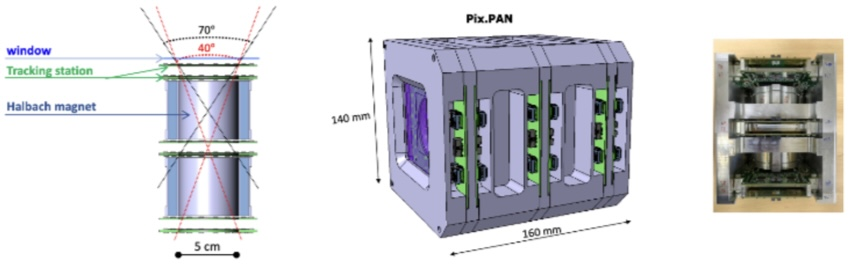
\includegraphics[width=1.0\textwidth]{FIGURES/LuPiX_PanPix.jpeg}
	\caption{A sketch of the layout of Pix.PAN,
showing the two magnet sectors and three tracking
stations. (Middle) Preliminary design of the mechanical
structure of the Pix.PAN spectrometer. (Right) The
Mini.PAN spectrometer demonstrator. From \cite{Wu2024}
	}
	\label{fig:LuPiX}
\end{figure}

